\documentclass[letterpaper,final,12pt,reqno]{amsart}

\usepackage[total={6.3in,9.2in},top=1.1in,left=1.1in]{geometry}

\usepackage{bm}
\usepackage{empheq}
\usepackage[dvipsnames]{xcolor}
\usepackage{graphicx}
\usepackage{verbatim,fancyvrb}
\usepackage{tikz}

% hyperref should be the last package we load
\usepackage[pdftex,
colorlinks=true,
plainpages=false, % only if colorlinks=true
linkcolor=blue,   % only if colorlinks=true
citecolor=Red,   % only if colorlinks=true
urlcolor=black     % only if colorlinks=true
]{hyperref}

\renewcommand{\baselinestretch}{1.05}

\newtheorem*{assumptions}{Assumptions}

\newcommand{\eps}{\epsilon}
\newcommand{\RR}{\mathbb{R}}

\newcommand{\grad}{\nabla}
\newcommand{\Div}{\nabla\cdot}
\newcommand{\sgn}{\operatorname{sgn}}
\newcommand{\spy}{\operatorname{spy}}
\newcommand{\trace}{\operatorname{tr}}

\newcommand{\bd}{\mathbf{d}}
\newcommand{\bg}{\mathbf{g}}
\newcommand{\bn}{\mathbf{n}}
\newcommand{\bu}{\mathbf{u}}
\newcommand{\bv}{\mathbf{v}}
\newcommand{\bx}{\mathbf{x}}

\newcommand{\bX}{\mathbf{X}}



\begin{document}
%\graphicspath{{figures/}}

\title[Synthetic, time-dependent glacier]{A synthetic, time-dependent glacier \\ for testing surface kinematical inversion}

\author{Ed Bueler}

\maketitle

%\vspace{-8mm}
\begin{center}
{\footnotesize
\emph{version: \today}}
\end{center}

\thispagestyle{empty}

\section{Surface kinematical equations}  This document describes in detail how the surface elevation, surface velocity, and surface mass balance of a synthetic glacier (or ice sheet) evolves.

We consider a flow-line with coordinates $x$ in the horizontal---there is only one horizontal dimension---and $z$ in the vertical.  Let $s(t,x)$ be the surface elevation.  (One may fix time $t$ and visualize $z=s(t,x)$ as a curve in the $x,z$ plane, or $z=s(t,x)$ can be visualized as a surface in $t,x,z$ space.)  Let $\bn_s(t,x) = \left<-\frac{\partial s}{\partial x},1\right>$ denote the upward normal vector on the ice surface; note that it is not a unit vector.  For simplicity the bed is flat ($b=0$), so the thickness and surface elevation coincide: $h=s$.

At the upper surface the ice has a velocity and the climate adds or removes ice.  Let $\bu(t,x,z)=\left<u,w\right>$ denote the ice velocity, with components $u$ in the horizontal and $w$ in the vertical.  Let $\bu|_s(t,x) = \bu(t,x,s(t,x)) = \left<u|_s,w|_s\right>$ denote the surface value of the ice velocity.  Let $a(t,x)$ be the climatic (surface) mass balance (CMB), also known as the accumulation-ablation function.

In these terms the traditional \emph{surface kinematical equation} (SKE), also called the ``kinematical boundary condition'' \cite{FowlerNg2021,GreveBlatter2009}, is
\begin{equation}
\frac{\partial s}{\partial t} - \bu|_s \cdot \bn_s - a = 0  \label{ske}
\end{equation}
This equation says that, at times $t$ and locations $x$ where ice is present, i.e.~$s(t,x)>0$, at the surface of the ice there is a balance between the rate of change of the surface elevation, the flow of the ice, and the CMB.  By expanding the dot product it is equivalent to write ``$\frac{\partial s}{\partial t} + u|_s \frac{\partial s}{\partial x} - w|_s - a = 0$'' or similar; such forms are seen in textbooks.

A new form of the same idea, the \emph{kinematical conservation law} (KCL), is integrated in time and space, and it applies everywhere.  That is, it applies not only on the surface of the ice but on the adjacent ice-free land.  The statement and derivation of this new form is in the early draft \cite{Bueler2022}.  Here we state it on a one-dimensional interval, $\Omega=[x_0,x_1]$, and an interval of time $[t_0,t_1]$:
\begin{align}
\frac{1}{2} \int_{x_0}^{x_1} h(t_1,x)^2\,dx &= \frac{1}{2} \int_{x_0}^{x_1} h(t_0,x)^2\,dx + \int_{t_0}^{t_1} \int_{x_0}^{x_1} \bu|_s(t,x)\cdot \bn_s(t,x)\,h(t,x) \,dx\,dt \label{kcl} \\
  &\hspace{34mm} + \int_{t_0}^{t_1} \int_{x_0}^{x_1} a(t,x)\,h(t,x) \,dx\,dt \notag
\end{align}
Equation \eqref{kcl} says that the square of the ice thickness, $h^2$, is conserved.  At a later time $t_1$ the total amount of $h^2$ is the same as at an earlier time $t_0$, except for identified and integrated contributions from ice dynamics ($=\int \int \bu|_s \cdot \bn_s\,h \,dx\,dt$) and CMB ($=\int \int a\,h \,dx\,dt$).  These contributions are ``weighted'' by the thickness, so thinner ice (small $h$) areas do not contribute much, and ice-free areas do not contribute at all.

The new form may be advantageous when we try to account for glacier changes in locations $x$ where the glacier is present at certain times ($h(t,x)>0$) and not at others ($h(t,x)=0$).  With the KCL there is no need to track the time-varying region occupied by the glacier, i.e.~the set $R(t) = \{x\,|\,h(t,x)>0\}$.  Equivalently, there is no need to know time-dependent glacier outlines.

We hope this new approach has advantages when inverting for the CMB function $a(t,x)$.  One should be able to simultaneously invert for the CMB, the equilibrium line altitude, and the time-dependent glacier outline from purely kinematical observations, namely of the surface elevation and the surface velocity.  (The ice thickness is also needed.)  However, this kind of inversion requires separating-out the vertical velocity at the surface $w|_s$.  In initial KCL inversion usage we will lump $w|_s$ with $a$, and we assume that we know surface elevation, slope, and horizontal velocity, supplemented by the $s=h$.

\begin{assumptions}  Fields $s(t,x)$, $\frac{\partial s}{\partial x}(t,x)$, and $u|_s(t,x)$ are observed at all points in $[t_0,t_1] \times [x_0,x_1]$.  The bed elevation is zero ($b=0$), and $s = \frac{\partial s}{\partial x} = u|_s =0$ at ice-free locations. \end{assumptions}

Putting the observed fields on the right and using $s=h$, we rewrite \eqref{kcl} as follows:
\begin{align}
\int_{t_0}^{t_1} \int_{x_0}^{x_1} s(t,x)\, \tilde a(t,x) \,dx\,dt &= \frac{1}{2} \int_{x_0}^{x_1} s(t_1,x)^2 - s(t_0,x)^2\,dx  \label{kclforinversion} \\
    &\quad + \int_{t_0}^{t_1} \int_{x_0}^{x_1} s(t,x)\, u|_s(t,x) \frac{\partial s}{\partial x}(t,x) \,dx\,dt \notag
\end{align}
where we will call
\begin{equation}
\tilde a(t,x) = w|_s(t,x) + a(t,x) \label{surfacerate}
\end{equation}
the \emph{lumped CMB}.

It is desirable to separate the two parts of $\tilde a$, but in initial usage it is easier to keep them together.  Techniques for evaluating $w|_s$, and thus separation of the CMB $a$ itself, are discussed in \cite{GudmundssonBauder1999}.  This topic forms a natural next step for the project.

Equation \eqref{kclforinversion} needs to be discretized into a linear matrix equation
\begin{equation}
M \bv = \bd \label{kcldiscrete}
\end{equation}
where $\bv$ is a vector of values of $\tilde a$ on a space-time grid.  Here $M$ and $\bd$ are formed by choosing time and space intervals over which to apply \eqref{kclforinversion}.  It is assumed that \eqref{kcldiscrete} will be an over-determined equation with $\bv\in\RR^n$, $\bd\in\RR^m$, and $m>n$.  This allows a least-squares solution which reduces sensitivity to noise in the observed fields.  Then a QR or SVD method will be used to solve for $\bv$, thus $\tilde a$.  The null space of the matrix $M$ represents the ice-free areas.  The glacier outline will arise from graphing $\tilde a$.

The details of constructing and using \eqref{kcldiscrete} are the content of the project.


\section{Synthetic glacier formulas}

The significance of the SKE and KCL, and of the above inversion proposal, will become clearer via construction of an exactly-specified, but synthetic, example.  This example has surface elevation, ice velocity, and CMB which evolve together in a manner so that the SKE and KCL are exactly satisfied.  (The SKE is exactly satisfied only in locations where it applies, of course.)

The specific synthetic geometry here is based on a steady-state ice sheet profile from section 5.3 of textbook \cite{vanderVeen2013}, called the \emph{Bueler profile} and introduced in \cite{Bueler2003}.  However, time dependence is added through making the center height and length time-varying, so the term $\frac{\partial s}{\partial t}$ is nonzero.  The relevant formulas, given next, use parameters from Table \ref{constantstable}.

\begin{table}
\begin{tabular}{clll}
variable  & description & units & value \\
\hline
$\spy$ & seconds per year &  & 31556926.0 \\
$A$ & ice softness in Glen law & $\text{Pa}^{-3}\,\text{s}^{-1}$ & $10^{-16}/\spy$ \\
$g$ & gravity & m s$^{-2}$ & 9.81 \\
$H_c^{(0)}$ & center height at time zero & m & 3000 \\
$L^{(0)}$ & glacier half-length at time zero & m & $400 \times 1000.0$ \\
$n$ & exponent in Glen flow law & & 3 \\
$q$ & derived (helper) power & & $q = 1+\frac{1}{n} = \frac{4}{3}$ \\
$r$ & \qquad '' & & $r = \frac{n}{2n+2} = \frac{3}{8}$ \\
$\rho$ & density of ice & kg m$^{-3}$ & 910 \\
$T$ & period of variation & s & $2000 \times \spy$
\end{tabular}
\bigskip
\caption{Values of constants.}
\label{constantstable}
\end{table}

\begin{figure}[t]
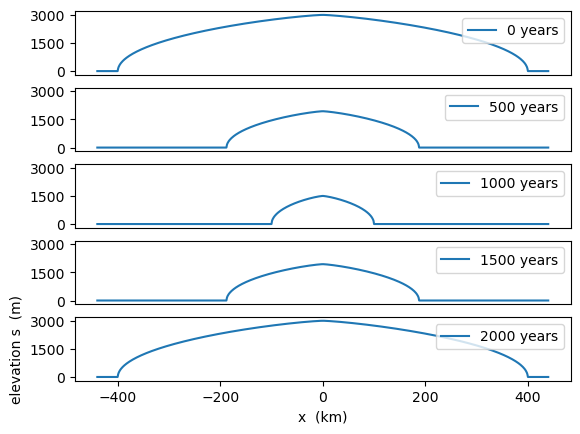
\includegraphics[width=0.85\textwidth]{surfacesnaps}
\caption{Surface elevation at five times in $0\le t \le 2000$ a.}
\label{surfacesnaps}
\end{figure}

First we define time-dependent surface elevation $s(t,x)$:
\begin{align}
H_c(t) &= H_c^{(0)} \left(1 - \frac{1}{2} \sin\left(\frac{\pi t}{T}\right)\right) \notag \\
L(t) &= L^{(0)} \left(1 - \frac{3}{4} \sin\left(\frac{\pi t}{T}\right)\right) \notag\\
\psi(t,x) &= (n+1) \frac{|x|}{L(t)} - 1 + n \left(1 - \frac{|x|}{L(t)}\right)^q - n \left(\frac{|x|}{L(t)}\right)^q \notag \\
s(t,x) &= H_c(t) (n-1)^{-r} \psi(t,x)^r \label{sformula}
\end{align}
See Figure \ref{surfacesnaps}.  The functions $H_c(t)$ and $L(t)$ determine how the center height and the glacier half-length, respectively, vary in time.  Formula \eqref{sformula} is the same as (5.50) in \cite{vanderVeen2013}, but made symmetric ($x \to |x|$), and with time dependence in $H_c$ and $L$.  Function $\psi(t,x)$ is simply a helper which simplifies certain formulas.  Note that $L(t)\ge \frac{1}{4} L_0 \ge 0$, thus $\psi(t,x)$ remains continuous despite the division in its definition.

The formula for $s(t,x)$ completely determines the evolution of the geometry of the glacier.  However, we need to compute the terms in equation \eqref{kclforinversion} in order to relate kinematic observations, of the surface elevation and velocity, to the lumped CMB $\tilde a(t,x)$.  For this purpose we will compute functions $\frac{\partial s}{\partial t}$, $\frac{\partial s}{\partial x}$, $u|_s$, and $\tilde a$ from \eqref{sformula}.

We start with the partial derivatives of $s(t,x)$:
\begin{align}
H_c'(t) &= - \frac{\pi H_c^{(0)}}{2T} \cos\left(\frac{\pi t}{T}\right) \notag\\
L'(t) &= - \frac{3 \pi L^{(0)}}{4T} \cos\left(\frac{\pi t}{T}\right) \notag \\
\phi(t,x) &= \left(1 - \frac{|x|}{L(t)}\right)^{1/n} + \left(\frac{|x|}{L(t)}\right)^{1/n} - 1 \notag \\
\frac{\partial \psi}{\partial t}(t,x) &= (n+1) \frac{L'(t)}{L(t)} \frac{|x|}{L(t)} \phi(t,x) \notag \\
\frac{\partial \psi}{\partial x}(t,x) &= - (n+1) \frac{\sgn(x)}{L(t)} \phi(t,x) \notag \\
\frac{\partial s}{\partial t}(t,x) &= (n-1)^{-r} \left[H_c'(t) \psi(t,x)^r + r H_c(t) \psi(t,x)^{r-1} \frac{\partial \psi}{\partial t}(t,x)\right] \label{dsdtformula} \\
\frac{\partial s}{\partial x}(t,x) &= r H_c(t) (n-1)^{-r} \psi(t,x)^{r-1} \frac{\partial \psi}{\partial x}(t,x) \label{dsdxformula}
\end{align}
Again, function $\phi(t,x)$ is merely a helper.  Notice that $\phi(t,0)=0$ and that $\phi(t,x)$ is continuous at $x=0$, and thus both $\frac{\partial \psi}{\partial t}$ and $\frac{\partial \psi}{\partial x}$ are continuous on the icy set $R = \{|x|<L(t)\}$.  (Specifically, $\frac{\partial \psi}{\partial t}(t,0)=\frac{\partial \psi}{\partial x}(t,0)=0$.)  It follows that $\frac{\partial s}{\partial t}$ and $\frac{\partial s}{\partial x}$ are also continuous on the icy set $R$.

The next step is a formula for the surface value of velocity.  This must come from assumptions about ice flow; it requires a choice of dynamics.  We will use the velocity generated from the shallow ice approximation (SIA), which also went into the construction of the original profile \cite[section 5.3]{vanderVeen2013}.  However, once we switch to inverting for CMB we will treat the surface velocity as observed, and its physical source will not matter.

An SIA formula gives the horizontal ice velocity as a function of the ice thickness, the surface elevation, and the $z$ coordinate.  (See \cite{GreveBlatter2009,vanderVeen2013} or equation (24) in my notes.)  Here the surface elevation and thickness are the same ($s=h$) so we may write:
\begin{equation}
u(t,x,z) = - \gamma \left(s(t,x)^{n+1} - (s(t,x)-z)^{n+1}\right) \left(\frac{\partial s}{\partial x}(t,x)\right)^n \label{siaxz}
\end{equation}
where $\gamma = 2 A (\rho g)^n / (n+1)$.  (Formula \eqref{siaxz}, without absolute values, is valid because $n$ is an odd integer.  We will only use $n=3$.)  The value at the surface comes from substituting $z=s(t,x)$:
\begin{equation}
u|_s(t,x) = - \gamma\, s(t,x)^{n+1} \left(\frac{\partial s}{\partial x}(t,x)\right)^n \label{siasurfacex}
\end{equation}
Using formulas \eqref{sformula} and \eqref{dsdxformula} allows the concrete computation of $u|_s(t,x)$.

Finally we may compute the lumped CMB $\tilde a(t,x) = w|_s(t,x) + a(t,x)$ by satisfying the SKE \eqref{ske}:
\begin{equation}
\tilde a(t,x) = \frac{\partial s}{\partial t}(t,x) + u|_s(t,x) \frac{\partial s}{\partial x}(t,x) \label{atildeformula}
\end{equation}
Applying formulas \eqref{sformula}, \eqref{dsdxformula}, and \eqref{siasurfacex} completes the concrete calculation.  Also observe that we could write
\begin{equation}
\tilde a(t,x) = \frac{\partial s}{\partial t}(t,x) - \gamma\, s(t,x)^{n+1} \left(\frac{\partial s}{\partial x}(t,x)\right)^{n+1} \label{atildefroms}
\end{equation}
That is, $\tilde a$ can be defined entirely in terms of the surface elevation $s$ and its derivatives.  Furthermore, when $n+1$ is an even integer, e.g.~since $n=3$, it follows that $\tilde a \le \frac{\partial s}{\partial t}$ on the ice surface.

The script \texttt{glacier.py} implements all of the above formulas.  See the \texttt{README.md} for documentation of usage in practice.

\small
\bigskip
\bibliography{synglac}
\bibliographystyle{siam}
\end{document}
